\documentclass[compress]{beamer}
%\documentclass[ignorenonframetext,handout]{beamer}
%\setbeamercovered{transparent}
%\usepackage[ISO 8859-1]{inputenc}
\usepackage{default}

% para usar figuras devemos acrescentar
\usepackage{graphicx}
%\usepackage{graphics}
%\DeclareGraphicsExtensions{.pdf,.png,.jpg}
%\DeclareGraphicsExtensions{.jpg, .eps}
%\DeclareGraphicsRule{.jpg}{eps}{.jpg}{`jpeg2ps -h -r 600 #1}
\usepackage{tikz}
%\usetikzlibrary{arrows,backgrounds,coordinatesystems,3d,shapes,plotmarks,automata,calendar,er,
%folding,matrix,mindmap,patterns,petri,plothandlers,topaths,trees} 
\usetikzlibrary{positioning}
%\usepgflibrary{decorations.pathreplacing}
\usetikzlibrary{decorations.pathreplacing}
\usetikzlibrary{decorations.pathmorphing}
\usetikzlibrary[patterns]
%\tikzstyle{every text node part}
%\usetikzlibrary{arrows,backgrounds,positioning,fit} 
\usetikzlibrary{calc}
% para gerar graficos no latex
\usepackage{pgfplots}
\pgfplotsset{compat=newest}

\usepackage{amsfonts}
\usepackage{amssymb}
\usepackage{amsmath}
\usepackage{MnSymbol}
\usepackage{amsmath}

\usepackage[brazil]{babel}
\usepackage[utf8]{inputenc}

% \usepackage{algpseudocode}
% \usepackage{algorithmicx}
\usepackage[Algoritmo]{algorithm}
\usepackage[noend]{algorithmic}

\setbeamertemplate{bibliography entry title}{}
\setbeamertemplate{bibliography entry location}{}
\setbeamertemplate{bibliography entry note}{}

\newcounter{saveenumi}
\newcommand{\seti}{\setcounter{saveenumi}{\value{enumi}}}
\newcommand{\conti}{\setcounter{enumi}{\value{saveenumi}}}

%\usepackage{shadethm}

%\definecolor{shadethmcolor}{rgb}{.75,.75,.75}

%\newshadetheorem{theorem}{\scshape Teorema}[chapter]
\newtheorem{teorema}[theorem]{\scshape Teorema}
\newtheorem{proposicao}[theorem]{\scshape Proposição}
\newtheorem{corolario}[theorem]{\scshape Corolário}
\newtheorem{lema}[theorem]{\scshape Lema}
\newtheorem{definicao}[theorem]{\scshape Definição}
\newtheorem{conjectura}[theorem]{\scshape Conjectura}
\newtheorem{escolio}[theorem]{\scshape Escólio}
\newtheorem{exemplo}[theorem]{\scshape Exemplo}
\newtheorem{exemplos}[theorem]{\scshape Exemplos}
\newtheorem{propriedade}[theorem]{\scshape Propriedade}

\renewcommand{\u}{{\bf u}}
\renewcommand{\v}{{\bf v}}
\renewcommand{\sin}{\operatorname{sen}}
\renewcommand{\tan}{\operatorname{tg}}
\providecommand{\cas}{\operatorname{cas}}
\providecommand{\mdc}{\mathrm{mdc}}
\providecommand{\f}{{\bf f}}

\newcommand{\ie}{\textit{i.e.}}
\newcommand{\eg}{\textit{e.g.}}
%\newcommand{\qed}{\hfill $\square$}

\renewcommand\Re{\operatorname{Re}}
\renewcommand\Im{\operatorname{Im}}

\providecommand{\x}{{\bf x}}
\providecommand{\y}{{\bf y}}
\providecommand{\w}{{\bf w}}
\providecommand{\f}{{\bf f}}
\providecommand{\q}{{\bf q}}
\providecommand{\bfa}{{\bf a}}
\providecommand{\bfb}{{\bf b}}
\providecommand{\bfc}{{\bf c}}
\providecommand{\bfd}{{\bf d}}
\providecommand{\bfe}{{\bf e}}
\providecommand{\bfs}{{\bf s}}
\providecommand{\bfz}{{\bf z}}
\providecommand{\zero}{{\bf 0}}
\providecommand{\spn}{\mathrm{span}}
\providecommand{\posto}{\mathrm{posto}}
\providecommand{\nul}{\mathrm{nul}}
\providecommand{\proj}{\mathrm{proj}}
\providecommand{\tr}{\mathrm{tr}}
\providecommand{\sgn}{\mathrm{sgn}}

\providecommand{\cov}{\mathrm{cov}}

\providecommand{\dilation}{\mathcal{D}}
\providecommand{\erosion}{\mathcal{E}}
\providecommand{\open}{\mathcal{O}}
\providecommand{\close}{\mathcal{C}}

\newcommand*{\Bhat}{\skew{3}{\hat}{B}}

\mode<presentation>
{
  \setbeamertemplate{background canvas}[vertical shading][bottom=white!10,top=blue!10]
%  \usetheme{Berkeley}
%  \usetheme{CambridgeUS}
%  \usetheme{Madrid}
  \usetheme{Warsaw}
  \usefonttheme[onlysmall]{structurebold}
  
  \setbeamertemplate{headline}{}
  
%   \setbeamercovered{invisible} % default
  \setbeamercovered{ transparent, again covered={\opaqueness{25}} } % =15%
%   \setbeamercovered{transparent=50}
%   \setbeamercovered{dynamic}

%   \setbeamercovered{again covered={\opaqueness<1->{25}}}
}

% copiado do site:
% http://latex-beamer-class.10966.n7.nabble.com/Covering-images-transparent-i-e-dimmed-figures-td1504
% . html
\usepackage{ifthen}

\makeatletter
\newcommand{\includecoveredgraphics}[2][]{
    \ifthenelse{\the\beamer@coveringdepth=1}{
        \tikz
            \node[inner sep=0pt,outer sep=0pt,opacity=0.15]
                {\includegraphics[#1]{#2}};
    }{
        \tikz
            \node[inner sep=0pt,outer sep=0pt]
                {\includegraphics[#1]{#2}};%
    }
} 
\makeatother % não sei se precisa...

%\pgfdeclareimage[height=1.4cm]{logo_XIVsm}{semanauniversitaria}

%% put XIVsm logo in bottom left
%\setbeamertemplate{sidebar left}{
%%   \vfill%
 %  \rlap{\hskip0.0cm
  %       %\href{http://www.uece.br/semanauniversitaria}
   %      {\pgfuseimage{logo_XIVsm}}}
   %%\vskip2pt%
   %%\llap{\usebeamertemplate***{navigation symbols}\hskip0.1cm}%
   %%\vskip2pt%
%}

% para a disciplina de Processamento de Imagens
\title{Inteligência Artificial\\Redes Neurais}
\author{Marlon Henry Schweigert}
\date{Semestre 2018-1}



\begin{document}


\frame{\titlepage}

%%%%%%%%%%%%%%%%%%%%%%%%%%%%%%

\section{Fonte Biológica}

\begin{frame}{Motivação}
    Primeiro neurônio artificial criado em 1943 utilizando circuitos elétricos~\cite{Yadav2015}.
\end{frame}

\begin{frame}{Motivação}
    Snark foi o primeiro neuro computador (1953) a processar utilizando redes neurais com ajuste de pesos. Porém, nunca processou uma função interessante~\cite{Yadav2015}.
\end{frame}

\begin{frame}{Motivação}
    1956 no Darthmouth College criou o neurônio Perceptron, programável~\cite{Yadav2015}.
\end{frame}

\begin{frame}{Motivação}
    \begin{figure}[h]
        
\includegraphics[height=7.5cm]{img/if.jpeg}
    \end{figure}
\end{frame}

\begin{frame}{Introdução}
    Redes Neurais tem o embasamento teórico de processamento do sistema nervoso biológico.
\end{frame}

\begin{frame}{Neurônio}
    Células especificadas em conduzir energia podendo alterar as características dos impulsos conduzidos\cite{Netter2015}.
\end{frame}

\begin{frame}{Neurônio}
    \begin{figure}[h]
        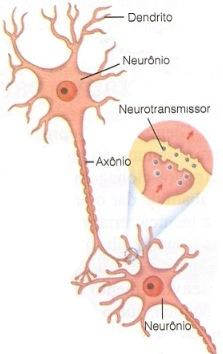
\includegraphics[height=7.5cm]{img/sinapse.jpg}
    \end{figure}
\end{frame}

\begin{frame}{Neurônio}
    \begin{figure}[h]
        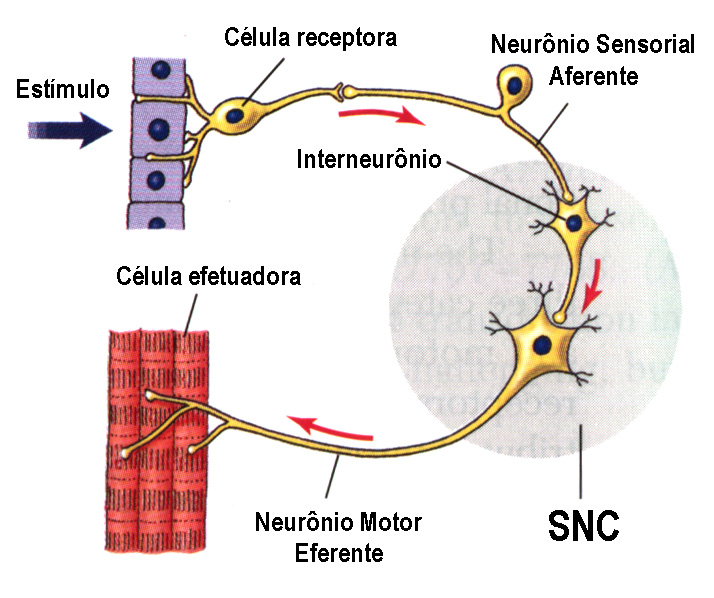
\includegraphics[height=7.5cm]{img/comunicacao.jpg}
    \end{figure}
\end{frame}

\section{Neurônio Computacional}

\begin{frame}{Modelo Matemático}
    \begin{figure}[h]
        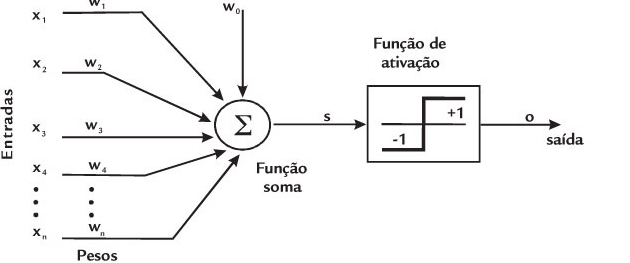
\includegraphics[height=4.5cm]{img/neuronio.png}
        
        Neurônio Perceptron\cite{Rosa2012Jun}.
    \end{figure}
\end{frame}

\begin{frame}{Modelo Matemático}
    \begin{itemize}
        \item Entradas $w_n$: Entrada de dados do neurônio, seja um vetor de dados ou outros neurônios (Rede multicamada).
        \item Entrada estável (bias): Constante de entrada para ter um valor padrão em caso de entrada nula. No neurônio Perceptron torna-se padrão a constante $-1$.
        \item Função soma: Função que agregará todas as entradas em um valor único $s$.
        \item Função de ativação: Função que tratará a entrada $u$ a fim de retornar uma resposta para outro neurônio ou retorno ao sistema.
    \end{itemize}
\end{frame}


\begin{frame}{Funções de Ativação}
    \begin{itemize}
        \item Função Degrau:
        $g(u)=$
        \begin{cases}
            1 se ($u\geq0$)\\
            0 se ($u$<$0$)
        \end{cases}
        
        \item Função Bipolar:
        $g(u)=$
        \begin{cases}
            1 se ($u$>$0$)\\
            0 se ($u$=$0$)\\
            -1 se ($u$<$0$)
        \end{cases}
        ou \begin{cases}
            1 se ($u\geq0$)\\
            -1 se ($u$<$0$)
        \end{cases}
    \end{itemize}
\end{frame}


\begin{frame}{Funções de Ativação}
    \begin{itemize}
        \item Função Logística:
        $g(u)=\frac{1}{1 + e^{-bu}}$, onde b é constante
        \item Função Tangente Hiperbólico:
        $g(u)=\frac{e^u  - e^-u}{e^u + e^-u}$
    \end{itemize}
\end{frame}

\begin{frame}{Rede Neural}
    \begin{figure}[h]
        
\includegraphics[height=4.5cm]{img/Brainslug.jpg}
    \end{figure}
\end{frame}

\begin{frame}{Rede Neural}
    \begin{figure}[h]
        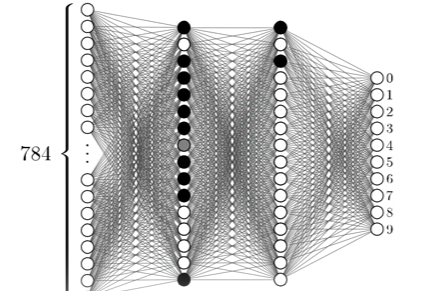
\includegraphics[height=4.5cm]{img/network.png}
        
        Modelo para reconhecimento de caracteres numéricas\cite{BibEntry2018Jun}.
    \end{figure}
\end{frame}

\begin{frame}{Rede Neural de múltiplas camadas}
    \begin{figure}[h]
        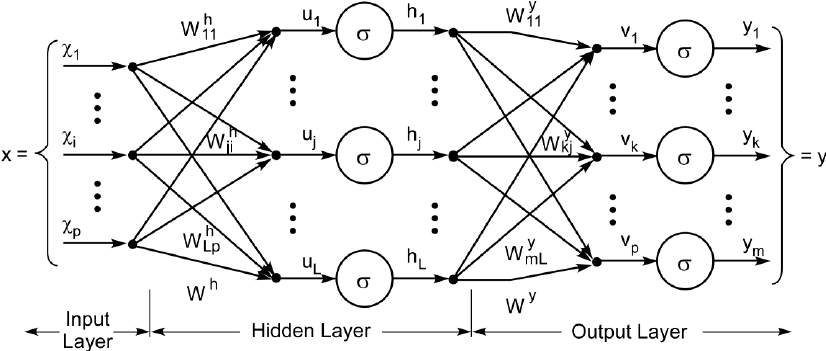
\includegraphics[height=4.5cm]{img/multilayer.png}
        
        Múltiplas camadas em uma rede neural\cite{BibEntry2018Jun2}.
    \end{figure}
\end{frame}

\begin{frame}{Modelagem Matricial}
    \begin{figure}[h]
        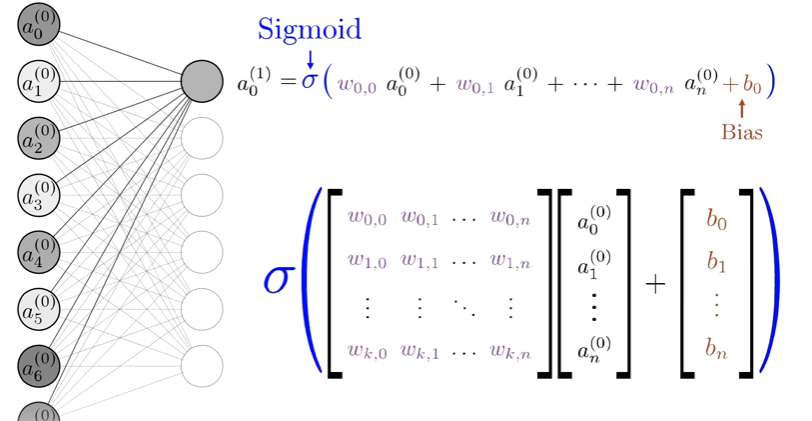
\includegraphics[height=4.5cm]{img/matrix.png}
        
        Produzindo sinapses com matrizes\cite{BibEntry2018Jun}.
    \end{figure}
\end{frame}

\begin{frame}{Como treinar?}
    Entradas de 28 por 28 pixels, em escala de cinza: $28x28(pesos) + 28(bias) = 812$ variáveis por camada.
    
    Como encontrar o valor de cada peso?~\cite{BibEntry2018May}
    
    \begin{enumerate}
        \item Regressão Linear
        \item Regressões Polinomiais
        \item Simulated Annealing
        \item Algoritmos Genéticos / Culturais
        \item Backpropagation
    \end{enumerate}
\end{frame}

\begin{frame}{Backpropagation}
    Como encontrar o erro?
    
    Como ajustar os erros das camadas anteriores utilizando este erro?
\end{frame}

\begin{frame}{Propagando correções aos pesos}
    $Err_n = V_e - V_r$, $V_e -> $ Vetor Esperado, $V_r ->$ Vetor Real
    
    Erro de cada nó:
    $Err_h = \frac{w_n}{\sum{w_i}} * \sum{Err_{h+1}}$~\cite{BibEntry2018}
    
    O erro é utilizado para atualizar o peso da sinapse com relação a um valor aleatório (opcional) e o Learning rate.
\end{frame}

\begin{frame}{Por onde começar?}
    Implementação manual? Talvez
    
    Frameworks? Tensorflow, Karas, etc
    
    Aplicações? Data Mining, Reconstrução de imagens (HyperGAN), Visão computacional, etc.
\end{frame}

\begin{frame}{Por onde começar?}
    \begin{figure}[h]
        
\includegraphics[height=4.5cm]{img/waiting.jpg}
    \end{figure}
    
    GPU: Processo de encontrar os pesos de uma rede neural é extremamente custoso.
\end{frame}

\begin{frame}{Onde utilizar?}
    \begin{enumerate}
        \item IA para jogos.
        \item Veículos autônomos.
        \item Reconhecimento de padrões.
        \item Classificação e recomendação.
        \item Reconstrução de dados.
        \item Avaliação de qualidade.
        \item Próteses cervo-nervosas.
        \item Gerar imagens de pokémon ou gatinhos
        \item Muito mais!
    \end{enumerate}
\end{frame}

\begin{frame}{Parte Prática}
    \begin{enumerate}
        \item \url{https://github.com/Schweigert/Pokemon_GAN} (MUITA GPU)
        \item
        \url{https://playground.tensorflow.org}
    \end{enumerate}
\end{frame}

%%% BIBLIOGRAFIA %%%
\begin{frame}[allowframebreaks]
\frametitle{Referências}
\bibliographystyle{plain}
\bibliography{ref.bib}
\end{frame}



\end{document}
